\section{Single-page Application (SPA)}
\Gls{spa} é uma implementação de aplicação web que carrega uma única página, um único arquivo do tipo \ac{html}, então de modo dinâmico modifica e atualiza o conteúdo da página de acordo com as ações do usuário, resultando em ganho de performance e melhor experiência de usuário. \cite{spamozilla}

Em uma \ac{spa} toda a codificação \ac{html}, JavaScript e \acs{css} é carregada de uma vez logo no primeiro acesso ou os recursos são recuperados (carregados) e incorporados à página conforme a necessidade, apenas o que for necessário, geralmente em resposta à interação do usuário \cite{wikispa}, como ilustrado na \autoref{spa-lifecycle}.

\begin{figure}[H]
	\centering
	\caption{\label{spa-lifecycle}Ciclo de vida: página web tradicional X \acs{spa}}
	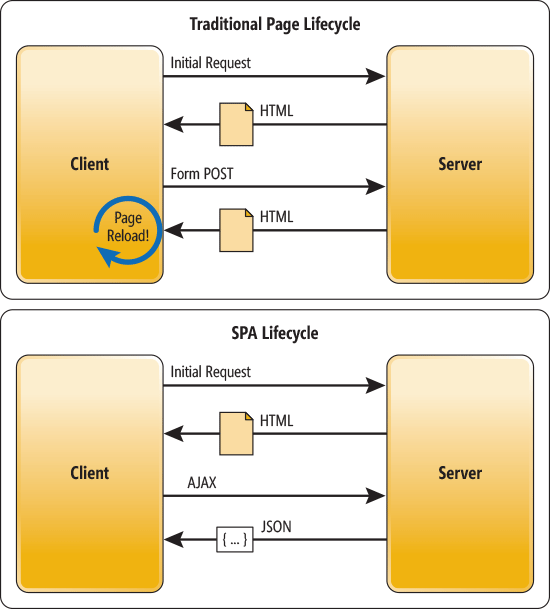
\includegraphics[width=0.50\textwidth]{../imagens/lit-spa-lifecycle.png}
	\fonte{\cite{fig_spa_lifecycle}}
\end{figure}